\section{Django}

\begin{frame}
\frametitle{Introduction to Django}
\begin{itemize}
\item Web development framework
\item Provides a set of resources for creating complex web applications 
  in an easy way
\item Development based on Python programming language and the
 Model-View-Controller pattern (MVC)
\item Open Source Project (BSD License)
\item \url{http://www.djangoproject.com}
\end{itemize}
\end{frame}

\begin{frame}
\frametitle{Model-View-Controller Pattern (MVC) (i)}
\begin{center}
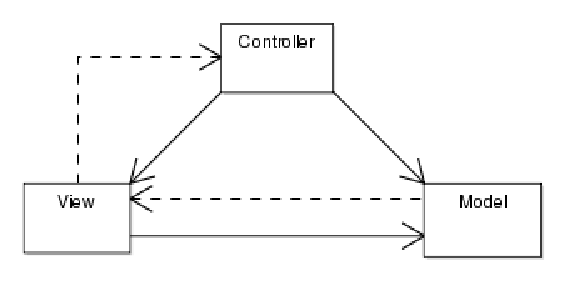
\includegraphics[width=10cm]{figs/MVC}
\end{center}
\end{frame}


\begin{frame}
\frametitle{Model-View-Controller Pattern (MVC) (ii)}
\begin{itemize}
\item \textbf{Model}: Representation of the data on which the application operates (raw data)
\item \textbf{View}: User interface
\item \textbf{Controller}: Manages the users requests and acts as exchanger between the model
  and the views.
\end{itemize}
\end{frame}


\begin{frame}[fragile]
\frametitle{Starting a Project}
\begin{itemize}
\item A \textbf{project} is a collection of settings for an instance of Django, including
  database configuration, Django-specific-options, and application-specific
  settings (\textit{Django Book})
\item An \textbf{application} is a portable set of Django functionality, 
   usually including models and views, that lives together in a single 
   Python package.
\item Initial commands
{\scriptsize
\begin{verbatim}
  django-admin.py startproject <PROJECT>
  django-admin.py startapp <APP>
  manage.py runserver [DOMAIN]
\end{verbatim}
}
\end{itemize}
\end{frame}


\begin{frame}
\frametitle{Introduction to DB Model}
\begin{itemize}
\item Data access layer
\item Supports several database storage engines (MySQL, PostgreSQL, SQLite, Oracle)
\item Access based on an ORM (Object Relational Mapper)
\item Suitable for object-programming 
\end{itemize}
\end{frame}


\begin{frame}[fragile]
\frametitle{Database Configuration}
\begin{itemize}
\item settings.py
{\scriptsize
\begin{verbatim}
  DATABASE_ENGINE = ""
  DATABASE_NAME = ""
  DATABASE_USER = ""
  DATABASE_PASSWORD = ""
  DATABASE_HOST = ""
  DATABASE_PORT = ""
\end{verbatim}
}
\end{itemize}
\end{frame}


\begin{frame}[fragile]
\frametitle{Useful DB commands }
\begin{itemize}
\item Validate model
{\scriptsize
\begin{verbatim}
  python manage.py validate
\end{verbatim}
}
\item Generate SQL
{\scriptsize
\begin{verbatim}
  python manage.py sqlall <app>
\end{verbatim}
}
\item Synchronize Model
{\scriptsize
\begin{verbatim}
  python manage.py syncdb
\end{verbatim}
}
\end{itemize}
\end{frame}


\begin{frame}[fragile]
\frametitle{Defining the Model}
\begin{itemize}
\item All classes inherit from models.Model
{\scriptsize
\begin{verbatim}
from django.db import models
   
class Author(models.Model):
  name = models.CharField(max_length=50)
  email = models.EmailField()
\end{verbatim}
}
\end{itemize}
\end{frame}


\begin{frame}[fragile]
\frametitle{Model Fields}
{\scriptsize
\begin{verbatim}
 - AutoField
 - CharField
 - TextField
 - IntegerField
 - FloatField
 - DateTimeField
 - BooleanField
\end{verbatim}
}
\end{frame}


\begin{frame}[fragile]
\frametitle{Model Relationships}
{\scriptsize
\begin{verbatim}
  ForeignKey(othermodel) -> 1-N
    a.fk = b
  OneToOneField(othermodel) -> 1-1 (FK with unique=True)
    a.fk = b
  ManyToManyField(othermodel) -> N-N
    a.fk.add(b)
\end{verbatim}
}
\end{frame}


\begin{frame}[fragile]
\frametitle{Model Field options}
{\scriptsize
\begin{verbatim}
  null=Boolean
  default=Type
  primary_key=Boolean
  unique=Boolean
  unique_for_date=Boolean
\end{verbatim}
}
\end{frame}

\begin{frame}[fragile]
\frametitle{Dealing with Model objects}
\begin{itemize}
\item Creating
{\scriptsize
\begin{verbatim}
a = Author(name='sduenas', ...)
a.save()
\end{verbatim}
}
\item Updating attributes
{\scriptsize
\begin{verbatim}
a.name = 'carlosgc'
a.save()
\end{verbatim}
}
\item Deleting
{\scriptsize
\begin{verbatim}
a.delete()
\end{verbatim}
}
\end{itemize}
\end{frame}

\begin{frame}[fragile]
\frametitle{Searching}
\begin{itemize}
\item Basic search
{\scriptsize
\begin{verbatim}
Author.objects.all()
Author.objects.get()
\end{verbatim}
}
\item Filters
{\scriptsize
\begin{verbatim}
Author.objects.filter(name="")
Author.objects.filter(name="Jesus", email__contains="libresoft.es")
Author.objects.order_by("name", "-email")
Author.objects.filter(name="").order_by("name")
\end{verbatim}
}
\end{itemize}
\end{frame}


%*********************************************************************
%*********************************************************************
%*********************************************************************

%\section{URLconfs}

\begin{frame}[fragile]
\frametitle{Introduction to URLconfs}
\begin{itemize}
\item Regular Expressions
\item Map URL patterns to views
{\scriptsize
\begin{verbatim}
from django.conf.urls.defaults import *

urlpatterns = patterns("",
  (r"^mysite/", include("mysite.urls")),
  (r"^admin/", include("django.contrib.admin.urls")),
)
\end{verbatim}
}
\end{itemize}
\end{frame}


\begin{frame}
\frametitle{Regular Expressions}
\begin{table}
\begin{small}
\centering
\begin{tabular}{|c|l|}
\hline
\textbf{Symbol} & \textbf{Meaning} \\
\hline
 . (dot) & any char \\
\hline
 * (dot) & 0 or more previous chars \\
\hline
 + (dot) & 1 or more previous chars \\
\hline
 ? (dot) & 0 or 1 previous char \\
\hline
 (?P<p>) & group and parameter \\
\hline
 [] & set of chars \\
\hline
{min,max} & range \\
\hline
\end{tabular}
\end{small}
\end{table}
\end{frame}


\begin{frame}[fragile]
\frametitle{URLconf Example}
{\scriptsize
\begin{verbatim}
 urlpatterns = patterns("",
   (r"^id/(?P<name>[A-Za-z\-]+)$", "mysite.views.id"),
   (r"^id/(?P<name>[A-Za-z\-]+)/auth/(?P<type>[a-z]+)$",
           "mysite.views.auths"),
   (r"^/num/(?P<num>d{2})$", "mysite.views.id"),
   (r"(?P<path>.*)$", "django.views.static.serve", 
      {"document_root": "/var/www/myproject/"},
 )
\end{verbatim}
}
\end{frame}


%*********************************************************************
%*********************************************************************
%*********************************************************************


\begin{frame}[fragile]
\frametitle{Views}
\begin{itemize}
\item Render template
{\scriptsize
\begin{verbatim}
render_to_response(<template>, <dict>)
\end{verbatim}
}
\item HttpResponse
{\scriptsize
\begin{verbatim}
HttpResponse(response, mimetype=<type>)
\end{verbatim}
}
\end{itemize}
\end{frame}

\begin{frame}[fragile]
\frametitle{Templates}
\begin{itemize}
\item Produce a dynamic text output requested by the user
\item Composed by text, variables (\{\{ var \}\}) and tags (\{\% tag \% \})
\item Context variables are passed from the view dictionary
\item Template and Context objects is also available
\end{itemize}
\end{frame}


\begin{frame}[fragile]
\frametitle{Tags (i)}
\begin{itemize}
\item \textit{if/else}
{\scriptsize
\begin{verbatim}

   <p>Found</p>

   <p>Not found</p>

\end{verbatim}
}
\item \textit{for}
{\scriptsize
\begin{verbatim}

   <p>{{day}}</p>

\end{verbatim}
}
\end{itemize}
\end{frame}


\begin{frame}[fragile]
\frametitle{Tags (ii)}
\begin{itemize}
\item \textit{include}
{\scriptsize
\begin{verbatim}

\end{verbatim}
}
\item \textit{block}
{\scriptsize
\begin{verbatim}

   <h1>Title</h1>

\end{verbatim}
}
\item \textit{extends}
{\scriptsize
\begin{verbatim}

\end{verbatim}
}
\end{itemize}
\end{frame}


%\section{More Django}

\begin{frame}
\frametitle{More on Django}
\begin{itemize}
\item Administration Site
\item Forms
\item Template Engine Extensions
\end{itemize}
\end{frame}


%\section{References}

\begin{frame}
\frametitle{References}
\begin{itemize}
\item \textit{Django Book} \url{http://www.djangobook.com/}
\item \textit{Django Documentation} \url{http://docs.djangoproject.com/en/dev/}
\end{itemize}
\end{frame}

